\documentclass{article}

\usepackage[T1]{fontenc}
\usepackage[utf8]{inputenc}
\usepackage[brazilian]{babel}
\usepackage{graphicx}
\usepackage[export]{adjustbox}[2011/08/13]
\usepackage{float}
\usepackage[pdftex]{hyperref}
\usepackage{epstopdf}
\usepackage{etoolbox}
\usepackage{amsmath}
\usepackage{amsfonts}
\usepackage{amssymb}
\usepackage{caption}
\usepackage{subcaption}
\usepackage{setspace}
\usepackage{tikz}
\usepackage{listings}
\usepackage{xcolor} 

\bibliographystyle{eric}
\patchcmd{\thebibliography}{\section*}{\section}{}{}


\newcommand{\R}{\ensuremath{\mathbb{R}}}
\newcommand{\Prob}{\ensuremath{\mathbb{P}}}
\newcommand{\K}{\ensuremath{\mathbb{K}}}
\newcommand{\U}{\ensuremath{\mathbb{U}}}
\newcommand{\N}{\ensuremath{\mathbb{N}}}
\newcommand{\Lg}{\ensuremath{\mathbb{L}}}
\newcommand{\T}{\ensuremath{\rm Tr}}
\newcommand{\sg}{{\sigma(x_k)}}

\newcommand{\G}{\ensuremath{\mathcal{G}}}
\newcommand{\F}{\ensuremath{\mathcal{F}}}
\newcommand{\C}{\ensuremath{\mathcal{C}}}
\newcommand{\E}{\ensuremath{\mathcal{E}}}
\newcommand{\Hn}{\ensuremath{\mathcal{H}}}
\newcommand{\Hoo}{\ensuremath{\mathcal{H}_\infty}}
\newcommand{\Hop}{\ensuremath{\mathcal{H}_{op}}}
% --------------------------------------------------
\newtheorem{theo}{Teorema}
\newtheorem{exa}{Exemplo}
\newtheorem{lemm}{Lema}
\newtheorem{coro}{Corolário}
\newtheorem{defn}{Definição}[section]


\DeclareCaptionType{capequ}[Equação][]
\captionsetup[capequ]{labelformat=empty}

\begin{document}
\input{capa.tex}

\onehalfspacing
\section{Objetivos}
	Esse experimento tem como objetivo o estudo de um conversor DC-DC de topologia reversível (buck/boost) e o efeito do duty-cycle na sua tensão de saída.

	% Resposta de uma das perguntas, depois ver onde colocar
	Para medir a corrente no indutor, utilizamos o sensor ACS756 da Allegro MicroSystems, cujo funcionamento encontra-se detalhado em \cite{bb:allegro}, disponível na placa didática. Esse sensor funciona através de um pequeno trecho condutivo acoplado a um circuito de efeito Hall. Quando existe corrente passando pelo condutor, o circuito Hall converte o campo magnético gerado em uma tensão de saída. Para converter essa tensão em corrente, devemos subtraí-la da metade do valor da tensão de alimentação fornecida ao IC (nominalmente $5\ V$ e supomos que essa é a maneira que o aparelho está montado no kit didático) e dividir ela pela sensibilidade do aparelho (podendo ser 20 ou 40 mV/A dependendo do tipo do IC, supomos que o utilizado tenha sensibilidade de 40 mV/A por falta de mais informações). Esse tipo de sensor é mais eficiente energeticamente e interfere menos no circuito medido do que uma resistência de medição interferiria.
\section{Conversor Buck}
Conectamos o kit didático para trabalhar e modo step-down conforme detalhado na figura \ref{fig:buesq}.
\begin{figure}[H]
	\centering
	\includegraphics[width=0.5\linewidth]{Dados/buck/esq}
	\caption{Conexões do chopper reversível em modo step-down \cite{bb:paiva}}
	\label{fig:buesq}
\end{figure}
Com $V_s = 12V$ e o sinal $TTL$ um trem de pulsos de $0$ a $5V$ DC com frequência de $3kHz$ e duty-cycle de $50\%$.

Medimos então a curva de corrente no indutor através do sensor ACS756 que pode ser visualizada na figura \ref{fig:buil}
\begin{figure}[H]
	\centering
	\includegraphics[width=0.5\linewidth]{Dados/buck/il}
	\caption{Curvas de corrente no indutor para conversor buck}
	\label{fig:buil}
\end{figure}
Como podemos ver estamos operando em modo de condução descontínua (a corrente no indutor chega a 0). O valor médio assumido pela corrente no indutor foi de aproximadamente $0.25 A$

Medimos também a tensão de saída do conversor, apresentada na figura \ref{fig:but3k}
\begin{figure}[H]
	\centering
	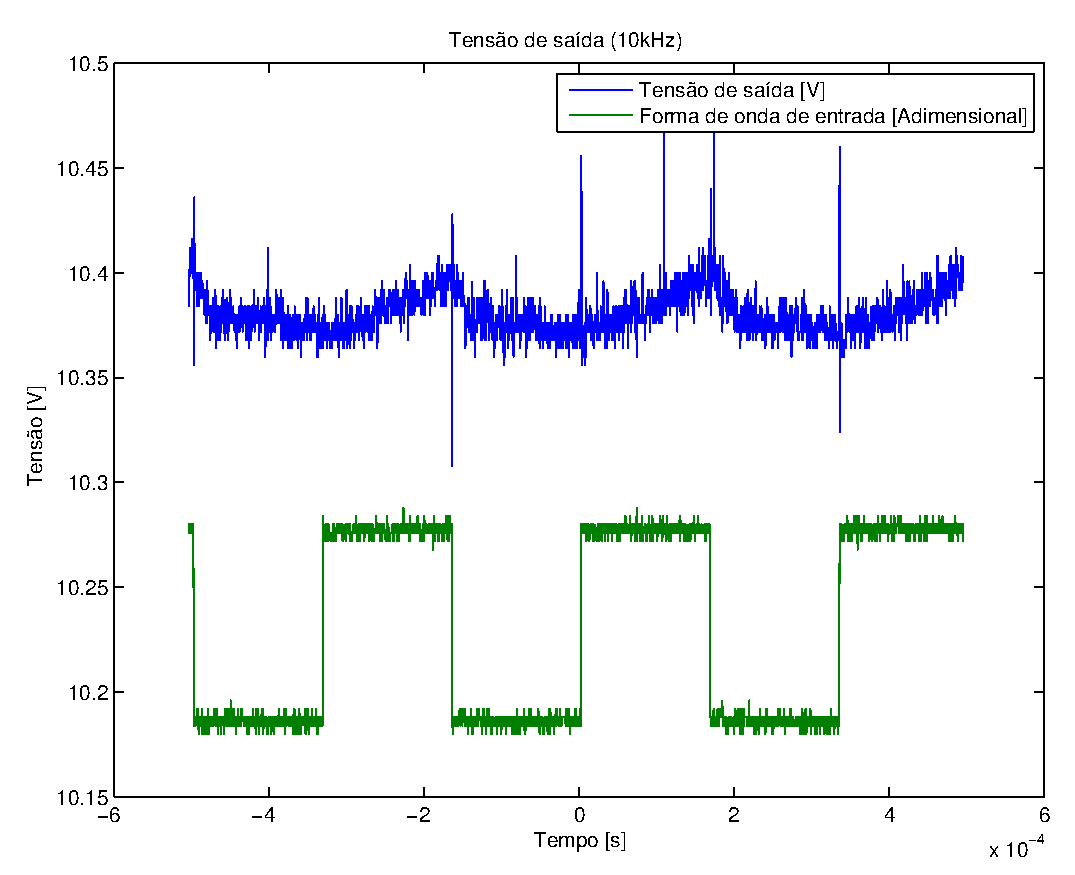
\includegraphics[width=0.5\linewidth]{Dados/buck/t3k}
	\caption{Tensão de saída conversor buck (3 kHz)}
	\label{fig:but3k}
\end{figure}

O valor médio da tensão de saída foi de $10.3 V$. Armados desses dados, do conhecimento de que o conversor estava trabalhando em modo de condução descontínua e da equação \ref{eq:bud} encontramos o valor da indutância de nosso kit didático: $L \approx 330.1 \mu H$

\begin{capequ}
	\begin{equation}
	\overline{V_R} = V_s\frac{D^2}{D^2 + 2\frac{LI_l}{V_s}}
	\end{equation}
	\caption{Equação da tensão de saída para conversor buck em modo de condução descontínua}
	\label{eq:bud}
\end{capequ}

Variamos o duty-cycle do sinal de controle entre $10$ e $70\%$ e medimos a tensão média sobre a carga. Encontramos uma curva que se aproxima desse sinal e que possuí a mesma forma da equação \ref{eq:bud} (equação \ref{eq:bulin}) e calculamos os valores teóricos que essa tensão deveria assumir (supondo modo de condução descontínua e que a corrente média no indutor se manteve aproximadamente $0.25 A$). Os resultados podem ser visualizados na figura \ref{fig:butvd}.

\begin{capequ}
	\begin{equation}
	V_R = 11.36\frac{D^2}{D^2 +  0.02055}	
	\end{equation}
	\caption{Curva que aproxima a tensão medida de saída em função do duty-cycle}
	\label{eq:bulin}
\end{capequ}

\begin{figure}[H]
	\centering
	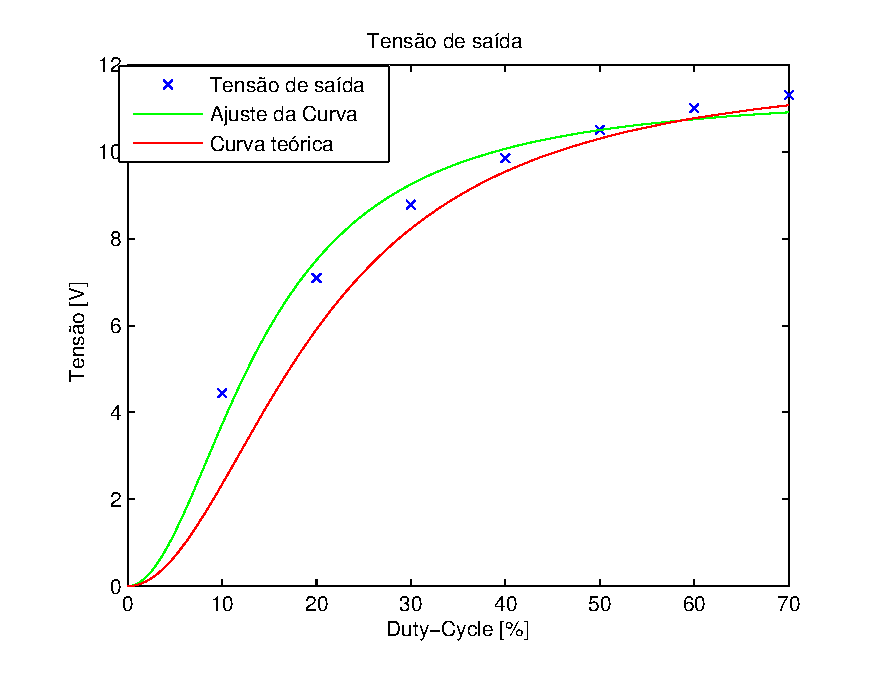
\includegraphics[width=0.7\linewidth]{Dados/buck/tvd}
	\caption{Tensão de saída conversor buck em função do duty-cycle}
	\label{fig:butvd}
\end{figure}

Como podemos ver os valores medidos estão bastante próximos dos esperados teoricamente porém levemente maiores. Isso acontece porque nos cálculos teóricos deixamos de levar em conta uma série de fatores, entre eles o fato dos componentes do circuíto não serem ideais (perdemos energia em vários pontos que não foram levados em conta), o fato da corrente média no indutor variar (fator que ignoramos para simplificar/possibilitar os cálculos), o fato de que a resposta dos componentes nem sempre é imediata entre outros. Também devemos lembrar que existem imprecisões de medida que afetam os resultados obtidos.

\section{Conversor Boost}

Conectamos o kit didático para trabalhar e modo step-up conforme detalhado na figura \ref{fig:boesq}.
\begin{figure}[H]
	\centering
	\includegraphics[width=0.5\linewidth]{Dados/boost/esq}
	\caption{Conexões do chopper reversível em modo step-up \cite{bb:paiva}}
	\label{fig:boesq}
\end{figure}
Com $V_s = 5V$ e o sinal $TTL$ um trem de pulsos de $0$ a $5V$ DC com frequência de $3kHz$ e duty-cycle de $50\%$.

Medimos então a curva de corrente no indutor através do sensor ACS756 que pode ser visualizada na figura \ref{fig:boil}
\begin{figure}[H]
	\centering
	\includegraphics[width=0.5\linewidth]{Dados/boost/il}
	\caption{Curvas de corrente no indutor para conversor boost}
	\label{fig:boil}
\end{figure}
Como podemos ver estamos operando em modo de condução contínua (a corrente no indutor não chega a 0).

Medimos também a tensão de saída do conversor, apresentada na figura \ref{fig:bot3k}
\begin{figure}[H]
	\centering
	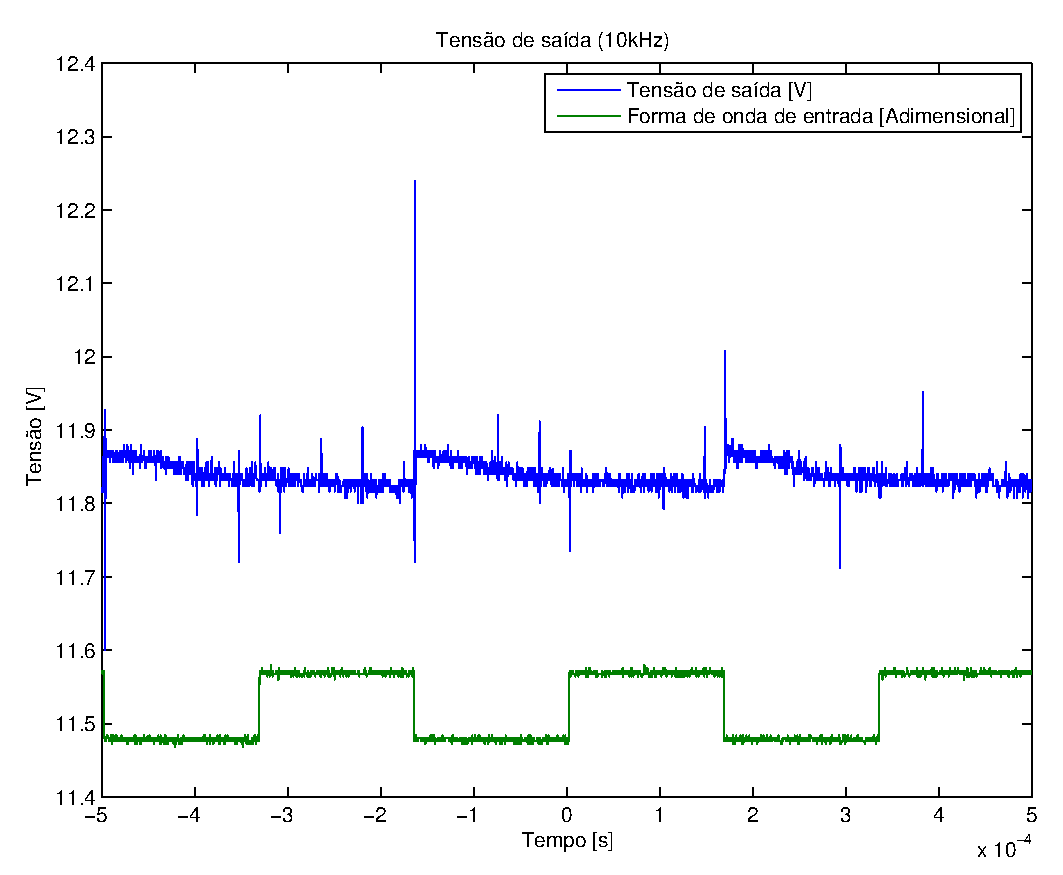
\includegraphics[width=0.5\linewidth]{Dados/boost/t3k}
	\caption{Tensão de saída conversor boost (3 kHz)}
	\label{fig:bot3k}
\end{figure}

O valor médio da tensão de saída foi de $11.9 V$.

Variamos o duty-cycle do sinal de controle entre $20$ e $70\%$ e medimos a tensão média sobre a carga. Encontramos uma curva que se aproxima desse sinal (equação \ref{eq:bolin}) e calculamos os valores teóricos que essa tensão deveria assumir (supondo modo de condução contínua). Os resultados podem ser visualizados na figura \ref{fig:botvd}.

\begin{capequ}
	\begin{equation}
	V_R = \frac{4.623}{1.011 - D}	
	\end{equation}
	\caption{Curva que aproxima a tensão medida de saída em função do duty-cycle}
	\label{eq:bolin}
\end{capequ}

\begin{figure}[H]
	\centering
	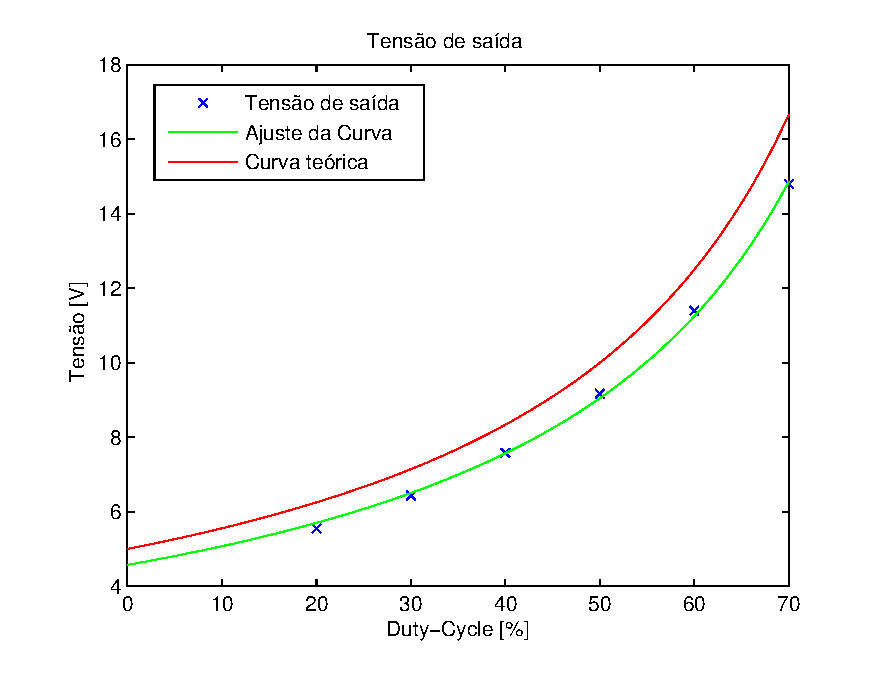
\includegraphics[width=0.7\linewidth]{Dados/boost/tvd}
	\caption{Tensão de saída conversor boost em função do duty-cycle}
	\label{fig:botvd}
\end{figure}

Como podemos ver os valores medidos estão bastante próximos dos esperados teoricamente porém levemente menores. Isso acontece porque nos cálculos teóricos deixamos de levar em conta uma série de fatores, entre eles o fato dos componentes do circuíto não serem ideais (perdemos energia em vários pontos que não foram levados em conta) e o fato de que a resposta dos componentes nem sempre é imediata. Também devemos lembrar que existem imprecisões de medida que afetam os resultados obtidos.

\bibliography{mybib}
\end{document}

